\chapter{Discussion}
\label{cap:discussion}
% \epigraphhead[50]{%
%     \epigraph{"if I have seen further it is by standing on the shoulders of Giants."}{Isaac Newton, 1675}
% }
\todo[inline]{TODO: Review by Mr Isaiah}
\subsection{Problem Formulation}
What if in a graph of connected components $G[\tilde{S}]$, the maximum number of nodes in a connected components are equal? This may not necessarily imply that the cost of disconnectivity (pairwise connectivity as a measure, say) is the same for all disconnected components. Therefore, might not solve the problem of disconnectivity in a network breakdown.
\begin{figure}[htb!]
\centering 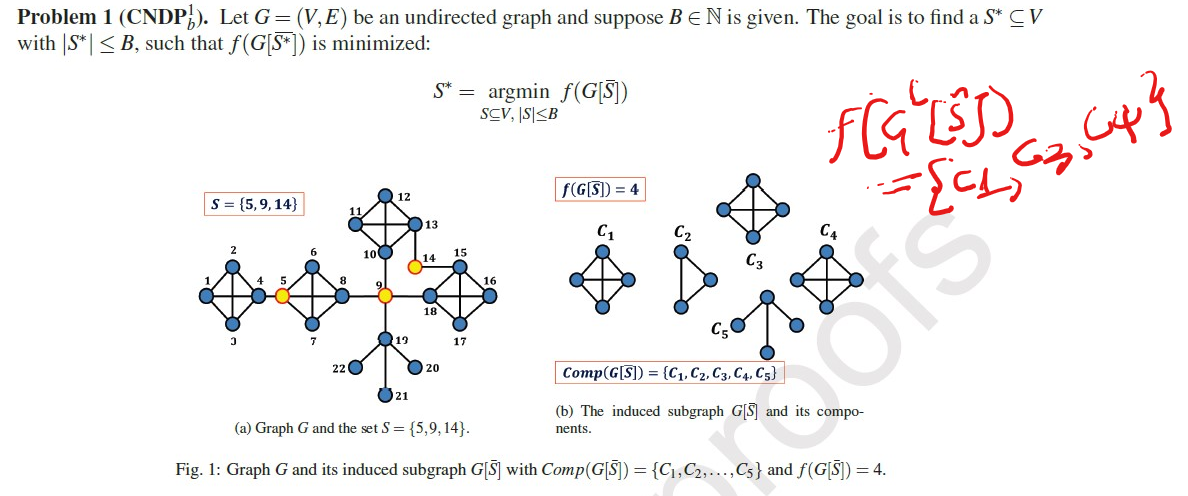
\includegraphics[width=\textwidth]{graphics/conn_comp.png}
\caption{Components}
\label{fig:conn_comp}
\end{figure}
For example, in the Graph above ${c_1, c_3, c_4}$ (in red in \ref{fig:conn_comp}) all have same value of maximum number of connected nodes which may not have same cost should there be weights - representing capacities or resilience index - attached to each node.
\subsection{Possible way out}
What if we formulate our objectives in such a way that:
\begin{enumerate}
    \item It first seek the maximum number of connected nodes in the subgraph; then \label{obj_1}
    \item Picks the one with the relevant figure of pairwise connectivity? \label{obj_2}
\end{enumerate}
By \ref{obj_1}, we assume the authors default structure. By \ref{obj_2}, we are able to extend their work.
If we succeed, the novelty will be the consideration of a scheme that considers both problems simultaneously through a sequential algorithm that counts first and evaluates next. That is, we will be combining $CNDP_a^1$ and $CNDP_b^2$; see \ref{fig:cdnp} below as in \cite{rezaei2020eia}.
\begin{figure}[htb!]
\centering 
\includegraphics[width=\textwidth]{graphics/cndp.png}
\caption{CND Problem Types}
\label{fig:cdnp}
\end{figure}


\subsection{Challenges}
Can't say for now how the simulation will look like. I mean I cannot predict the feasibility. But if we agree on this objective, the formulation is quite "theoretically or mathematically" feasible and explainable. But theory do not always guarantee feasibility in programming.

% We inspired our work from \citet{Chakrabarti2014}.
% \acrshort{sysml} is the reference in this field \citep{ObjectManagementGroup2015}
% The tools keep evolving \citep{Skoltech2017}.

